In order to check for security vulnerabilities we first have to find a suitable way to represent a program. This representation has to contain specific information about the program to be able to answer questions about security vulnerabilities. The information we need in this dissertation is twofold:

\begin{enumerate}
\item A program can contain many branches, loops and other control structures. We need to know the exact order of execution along each path in the program before we can make assumptions about security vulnerabilities. Therefore information is needed about which functions can be applied at a call site. This type of information is called \textit{control flow}.
\item Variables in JavaScript are mutable, so their values can change at any moment in a program. \textit{Value flow} information tells us exactly what values an expression may evaluate to. This is very important w.r.t. security, as some harmless variable may become referenced to a malicious variable somewhere in the program. From there on, that variable should be marked as pointing to the same value as the malicious variable.
\end{enumerate}

Aside from the representation, some technique has to be found to efficiently express security checks in the form of user-specified, application specific security policies. A naive way to examine programs would be to run them and keep track of any relevant information along the execution. Not only would this be tiresome, we can also not guarantee that the program will ever terminate, that it terminates without errors, or that it will have the same outcome for different inputs. A better approach would be to to analyze the program without having to run it. To this extent, a technique called \textit{static analysis} can be used.

This chapter describes how static analysis can be used to examine programs and how this analysis can be addressed to obtain information about specific parts of a program. First, section \ref{sec:staticAnalysis} describes more precisely what static analysis is and how it is interesting for this dissertation. Next, We discuss some approaches using static analysis to find generic vulnerabilities in programs in section \ref{sec:genericVulnerabilities}. Finally, some application-specific approaches for checking security vulnerabilities are discussed. For these approaches we take a deeper look on how they query the information specified by the analyses they perform. We end this chapter by giving a brief conclusion.

\section{Introduction to static analysis}
\label{sec:staticAnalysis}
Rice's theorem tells us that there is no general or effective method to prove non-trivial properties about a program. This problem is similar to the halting problem, which is undecidable. \textit{Static analysis} is a technique for analyzing computer programs without having to execute them. In this way we can avoid the possible problems we might encounter using a naive technique, as described above. The results of the analysis indicate program defects or prove certain properties of the program. As proving non-trivial properties about a program is undecidable, static analysis focusses on the instances of the problem about which it can tell whether the program satisfies a property or not, and leaves other instances unsolved. The results of the static analysis will then be a useful set of approximate solutions. Figure \ref{fig:decider} shows the main difference between a regular decider, which will always provide an exact answser, and a static analyzer.

\begin{figure}[!h]
    \centering
      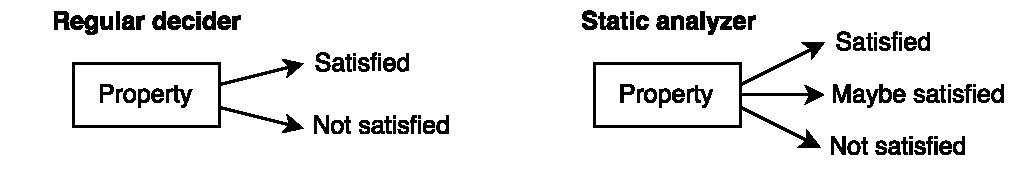
\includegraphics[width=0.9\textwidth]{images/decider} 
      \caption{Proving program properties: Regular decider and static analyzer}
    \label{fig:decider}
\end{figure}

\textit{Precision} is very important in static analysis. Consider a static analyzer that concludes for each property that it is \textit{maybe} satisfied. It is clear to see that there is no precision in this analysis, rendering it useless. We have to strive to attain enough precision to solve the maximum number of problem instances. \textit{Speed} on the other hand is less important for static analysis. As static analysis is decidable, it is guaranteed that the analysis will run in finite time, but gathering precise results is much more meaningful than the performance of the analysis itself. 
One particularly interesting technique used for static analysis is \textit{abstract interpretation}. This technique mimics interpretation of the program and allows to stay close to the original language semantics of those program without having to modify or instrument them to perform the analysis (in contrast to other static analysis techniques such as \textit{symbolic execution}). This mimicing of programs fits well for this dissertation, as we need to check for application-specific security vulnerabilities. It is thus a prerequisite that the semantics of the analyzed program lean as close to the original semantics as possible. A nice feature of abstract interpretation is that it allows to specify the precision needed by parameterizing it with a \textit{lattice}, but more on the topic of lattices follows in section \ref{subsec:lattice}. 

\subsection{Abstract interpretation}
%Quentin thesis
Abstract interpretation is a static analysis technique used to reason about a program. It does this by interpreting an approximation of a program through abstraction of its semantics. A \textit{sound} analysis can be performed and the precision of this analysis can be adjusted to the user's needs through various mechanisms. This increase in precision comes at the cost of a greater analysis running time. 

Abstract interpretation works in a similar way as normal program interpretation (so-called \textit{concrete interpretation}). The concrete interpretation of a program can be described as follows: 

\subsection{Lattices}
\section{Support for generic vulnerabilities}
\label{sec:genericVulnerabilities}
% Ref naar findbugs enzo (quentin thesis ook?)
% Nadeel fixed set, niet flexibel
\section{Support for application-specific vulnerabilities}
\label{sec:applicationSpecificVulnerabilities}
% PQL, GateKeeper, JunGL -> RPE OPHEMELEN
\section{Conclusion}
%State of the art in statische analyse staat ver genoeg op application-specific toer op te gaan & RPE zijn de manier waarop. Dit stuk moet overeenkomen met de motivatie